\subsection{Fault Treatment Patterns}


\begin{itemize}
	\item Wird ein Error mithilfe von \textbf{Detection Patterns} gefunden, wird das System entweder durch
	\begin{itemize}
		\item \textbf{Recovery Patterns} zurück in einen fehlerfreien Zustand überführt, oder der Error wird durch
		\item \textbf{Mitigation Patterns} maskiert, sodass die Auswirkungen so klein wie möglich gehalten werden
	\end{itemize}
	\item Nun kommen die \textbf{Fault Treatment Patterns} zum Einsatz; Es wird versucht, den Fault welcher den Error verursacht zu finden und zu korrigieren.
\end{itemize}



\begin{figure}[H]
	\centering
	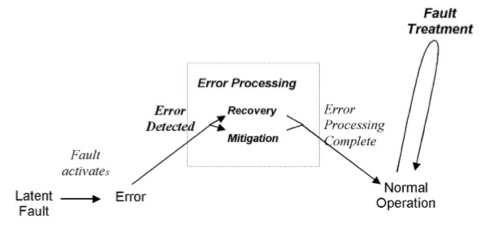
\includegraphics[width=\textwidth]{content/faulttolerance/images/fault_treatment.png}
	\caption{fault treatment}
\end{figure}




Um einen Fault mithilfe der \textbf{Fault Treatment Patterns} zu eliminieren, werden folgende Schritte durchloffen:
\begin{itemize}
	\item \textbf{Verification}
	\begin{itemize}
		\item Es wird geprüft, ob sich das System gemäss seiner Spezifikation verhält. Dies wird gemacht um zu prüfen, ob sich der Fault (immer noch) im System befindet.
	\end{itemize}
	\item \textbf{Diagnosis}
	\begin{itemize}
		\item Die Ursache des Fehlers wird untersucht. Es gilt, den Fault welcher zum Error führt, aufzuspüren und die genaue Erscheinungsform des Errors zu erforschen.
	\end{itemize}
	\item \textbf{Correction}
	\begin{itemize}
		\item Der Fehler wird aus dem System entfernt. (Sourcecode, System-Konfiguration etc.)
	\end{itemize}
	\item \textbf{Verification} \#2
\end{itemize}

\subsubsection*{Prüfungsfragen}

\begin{itemize}
	\item Was ist das Ziel von Fault Treatment Patterns?
	\item Welche Schritte werden beim Einsatz von Fault Treatment Patterns durchloffen?
\end{itemize}

